\documentclass[10pt,a4paper]{article}
\usepackage{rpgcover}
\usepackage{illustrated-panel}
\usepackage{longtable,booktabs}
\usepackage{float}
\usepackage{multicol}
\usepackage{fancyvrb}
\usepackage{wrapfig}
\usepackage{needspace}
\usepackage{titlesec}
\babelprovide[import]{spanish}
\selectlanguage{spanish}
\titleformat{\subsection}{\normalfont\Large\bfseries\color{rpgbrown}}{}{0pt}{}
\titlespacing*{\subsection}{0pt}{12pt plus 2pt}{5pt}
\titleformat{\subsubsection}{\normalfont\normalsize\bfseries\color{rpgbrown}}{}{0pt}{}
\titlespacing*{\subsubsection}{0pt}{10pt plus 2pt}{4pt}
\usepackage{etoolbox}
\pretocmd{\subsection}{\needspace{5\baselineskip}}{}{}
\pretocmd{\subsubsection}{\needspace{4\baselineskip}}{}{}
\setcounter{tocdepth}{1}
\clubpenalty=10000
\widowpenalty=10000
\displaywidowpenalty=10000
\interlinepenalty=0
\emergencystretch=1.2em
\newcommand{\HHInlineFigure}[3]{%
  \begin{center}\includegraphics[width=#2\linewidth,height=56mm,keepaspectratio]{assets/hollow-hearth/#1.png}%
  \par\vspace{2pt}{\footnotesize\itshape\color{rpgbrown}#3\par}\end{center}}
\newcommand{\HHSceneMap}[3]{%
  \clearpage\thispagestyle{rpg}%
  \vspace*{5mm}%
  \begin{center}
    {\Large\bfseries\color{rpgbrown}#2\par}\vspace{6mm}%
    \includegraphics[width=.96\linewidth,height=190mm,keepaspectratio]{assets/hollow-hearth/#1.png}\par\vspace{4mm}%
    {\small\itshape\color{rpgbrown}#3\par}%
  \end{center}%
  \clearpage}
\newcommand{\HHContents}{%
  \clearpage\thispagestyle{rpg}
  \vspace*{10mm}\begin{center}{\fontsize{27}{31}\selectfont\bfseries ÍNDICE\par}\vspace{9pt}
  {\color{rpgline}\rule{.76\linewidth}{.55pt}}\end{center}\vspace{9mm}
  \begingroup
  \expandafter\def\csname l@section\endcsname##1##2{\csname @dottedtocline\endcsname{1}{0em}{4em}{\bfseries ##1}{##2}}%
  \csname @starttoc\endcsname{toc}\endgroup
  \vspace{5mm}
  \begin{center}
\includegraphics[height=68mm,width=.59\linewidth,keepaspectratio]{assets/hollow-hearth/front-overlay.png}\end{center}
  \vfill
  \begin{center}{\small\itshape Una aventura de Jacopo Biscella\par}\vspace{5pt}
  {\footnotesize Esta aventura se distribuye bajo Creative Commons Atribución–CompartirIgual 4.0 Internacional (CC BY-SA 4.0), en las mismas condiciones que La última tirada. Se permite compartir y adaptar el material, incluso comercialmente, citando al autor y manteniendo la licencia en las obras derivadas.\par}\end{center}
  \clearpage}
\RPGSetRunningTitle{La campana de Hogar Hueco}
\RPGSetCoverWordSpace{.78em}
\hypersetup{pdftitle={La campana de Hogar Hueco},pdfauthor={Jacopo Biscella}}
\setlength{\emergencystretch}{2em}
\setcounter{secnumdepth}{-1}
\newcommand{\tightlist}{\setlength{\itemsep}{0pt}\setlength{\parskip}{0pt}}

\newcommand{\HHFrontArt}{assets/hollow-hearth/front-overlay.png}
\newcommand{\HHBackArt}{assets/hollow-hearth/back-overlay.png}
% Existing rpgcover.sty is used unchanged; only an adventure-specific back-cover layout follows.

\setlength{\parskip}{3.85pt plus .5pt minus .5pt}
\linespread{1.115}\selectfont
\newcommand{\HHAdventureBackCover}{%
 \clearpage\pagenumbering{gobble}\RPGCoverPagetrue\thispagestyle{empty}\null
 \begin{tikzpicture}[remember picture,overlay,x=1mm,y=1mm]
  \RPGDrawBackground{\RPGBackBackgroundFile}
  \node[align=center,text=coverink,text width=170mm,inner sep=0pt] at ($(current page.south west)+(105mm,260mm)$)
    {{\RPGCoverTitleFont\fontsize{19}{23}\selectfont LA CAMPANA DE HOGAR HUECO}};
  \draw[coverink,line width=.45pt] ($(current page.south west)+(57mm,246mm)$)--($(current page.south west)+(153mm,246mm)$);
  \node[anchor=north,align=left,text=coverink,text width=137mm,inner sep=0pt] at ($(current page.south west)+(105mm,240mm)$)
    {\RPGCoverTextFont\fontsize{10.4}{13.4}\selectfont
    Hace siete generaciones, un Místico errante bendijo una campana de bronce. La aldea donde termina el camino del rey y comienza el bosque se llamó Hogar Hueco. Al sonar al anochecer, la campana mantenía lejos a la Gente Hueca: criaturas pálidas de piel como corteza que susurran entre los árboles.};
  \node[anchor=north,align=center,text=coverink,text width=140mm,inner sep=0pt] at ($(current page.south west)+(105mm,197mm)$)
    {\RPGCoverSubtitleFont\fontsize{13}{17}\selectfont Hace tres noches robaron la campana.\\[4pt]
    La próxima noche sin luna llegará dentro de cuarenta y ocho horas.};
  \draw[coverink,line width=.45pt] ($(current page.south west)+(57mm,167mm)$)--($(current page.south west)+(153mm,167mm)$);
  \node[anchor=north,align=left,text=coverink,text width=137mm,inner sep=0pt] at ($(current page.south west)+(105mm,162mm)$)
    {\RPGCoverTextFont\fontsize{9.9}{12.1}\selectfont
    Una aventura introductoria para La última tirada, con tres o cuatro Protagonistas y una sesión de dos o tres horas. Enseña las tiradas por niveles, las distancias narrativas, la reserva de Heridas, la magia y la Reacción adversa, y el momento que da nombre al juego.};
  \node[anchor=north,align=center,text=coverink,text width=147mm,inner sep=0pt] at ($(current page.south west)+(105mm,133mm)$)
    {\RPGCoverSubtitleFont\fontsize{10.5}{13.2}\selectfont
     Tres opciones. Un final elegido por el grupo.\\
     Un caballero deshonrado. Un comprador que no es lo que parece.\\
     Una decisión que tomarán juntos.};
  \node[anchor=north,align=center,text=coverink,text width=144mm,inner sep=0pt] at ($(current page.south west)+(105mm,114mm)$)
    {\RPGCoverTextFont\fontsize{10.2}{12.5}\selectfont
     Incluye: cuatro mapas $\cdot$ cinco ilustraciones $\cdot$\\ una referencia rápida del Narrador con reglas y encuentros.};
  \RPGOptionalArtwork{105}{59}{130}{24}{\HHBackArt}
  \filldraw[fill=white,draw=coverink,line width=.55pt]
    ($(current page.south west)+(139mm,25mm)$) rectangle
    ($(current page.south west)+(187mm,55mm)$);
 \end{tikzpicture}
 \clearpage\RPGCoverPagefalse
}
\newcommand{\HHFrontCover}{%
 \clearpage\RPGCoverPagetrue\thispagestyle{empty}\null
 \begin{tikzpicture}[remember picture,overlay,x=1mm,y=1mm]
  \RPGDrawBackground{\RPGFrontBackgroundFile}
  \node[align=center,text=coverink,text width=138mm,inner sep=0pt]
   at ($(current page.south west)+(105mm,248mm)$)
   {\RPGCoverTitleFont\fontsize{16.6}{20.7}\selectfont LA CAMPANA DE\\[1.0mm]HOGAR HUECO};
  \node[align=center,text=coverink,text width=135mm,inner sep=0pt]
   at ($(current page.south west)+(105mm,235mm)$)
   {\RPGCoverSubtitleFont\fontsize{9.5}{12}\selectfont Una aventura para «La última tirada»};
  \RPGOptionalArtwork{105}{119}{150}{138}{\HHFrontArt}
  \node[align=center,text=coverink,text width=124mm,inner sep=0pt]
   at ($(current page.south west)+(105mm,25mm)$)
   {\RPGCoverTextFont\fontsize{12}{15}\selectfont Jacopo Biscella};
 \end{tikzpicture}\clearpage\RPGCoverPagefalse}
\begin{document}
\RPGStartFrontMatter
\HHFrontCover
\HHContents
\RPGStartMainMatter
\RPGChapter{La campana de Hogar Hueco}
\begin{center}\textit{Una aventura introductoria para La última tirada}\par\smallskip
\small 2--3 horas \textperiodcentered\ 3--4 Protagonistas \textperiodcentered\ Al menos un Guerrero \textperiodcentered\ Edición para el Narrador
\end{center}
\noindent\textit{Las cuatro hojas de personaje pregeneradas se ofrecerán en un PDF aparte, una hoja por Protagonista, con la plantilla de hoja de personaje del manual.}\par\medskip
\subsection{Unas palabras para el Narrador}\label{unas-palabras-para-el-narrador}

Esta aventura es, ante todo, una herramienta de aprendizaje y, después, una historia. Cada escena pone en primer plano un pilar concreto de \emph{La última tirada} sin detener nunca la ficción para dar lecciones. Cuando terminéis, tus jugadores habrán vivido las tiradas por niveles, las distancias narrativas, la reserva única de Heridas y Fatiga, la mecánica de Ayuda y, si haces bien tu trabajo, al menos un Esfuerzo declarado con mano temblorosa justo en el momento que promete el título.

El ritmo aproximado es:

\begin{itemize}
\tightlist
\item
  30 minutos para crear los personajes y preparar la partida \emph{(usa las reglas de creación del manual, págs. 2--6)}
\item
  35 minutos para \textbf{Escena 1 · La aldea} (investigación social)
\item
  40 minutos para \textbf{Escena 2 · El bosque susurrante} (prueba de habilidad y ambiente)
\item
  60 minutos para \textbf{Escena 3 · La antigua atalaya} (clímax de combate y desenlace)
\item
  10 minutos para \textbf{Las tres preguntas} y las consecuencias
\end{itemize}

Un recordatorio que conviene repetir: en este juego no hay tiradas de iniciativa, ni orden de turnos fijo, ni cuadrícula. Los mapas incluidos en esta aventura son anclas espaciales para la imaginación de todos; en la mesa, las distancias son siempre \textbf{Contacto}, \textbf{Cerca}, \textbf{A distancia} o \textbf{Lejos}.

\par\vspace{3pt}

\subsection{Qué enseña esta aventura}\label{quuxe9-enseuxf1a-la-aventura}

\begingroup\setlength{\arrayrulewidth}{.34pt}\arrayrulecolor{rpgline}\renewcommand{\arraystretch}{1.32}\rowcolors{2}{rpgshade}{white}\par\smallskip\noindent\begin{tabularx}{\linewidth}{|Y|Y}\hline
\rpghead{Escena} & \rpghead{Mecánicas introducidas} \\ \hline
La aldea & Tiradas de Atributo + Habilidad; NO de las acciones sociales; tiradas enfrentadas; uso del Rasgo y la Carga \\ \hline
El bosque susurrante & Ayuda; Condiciones ($-1$ grado); categorías de distancia narrativas \\ \hline
La antigua atalaya & Combate; Heridas y Fatiga; Crítico; Reacción adversa; \textbf{Esfuerzo}; consecuencias \\ \hline
\end{tabularx}\arrayrulecolor{black}\endgroup\par\smallskip

Si el grupo incluye un Místico, la tercera escena es también donde probablemente sufrirá su primera Reacción adversa. Deja que ocurra.

\par\vspace{3pt}

\par\needspace{65mm}\subsection{La premisa}\label{la-premisa}

\begin{wrapfigure}{r}{.38\linewidth}\vspace{-5pt}\centering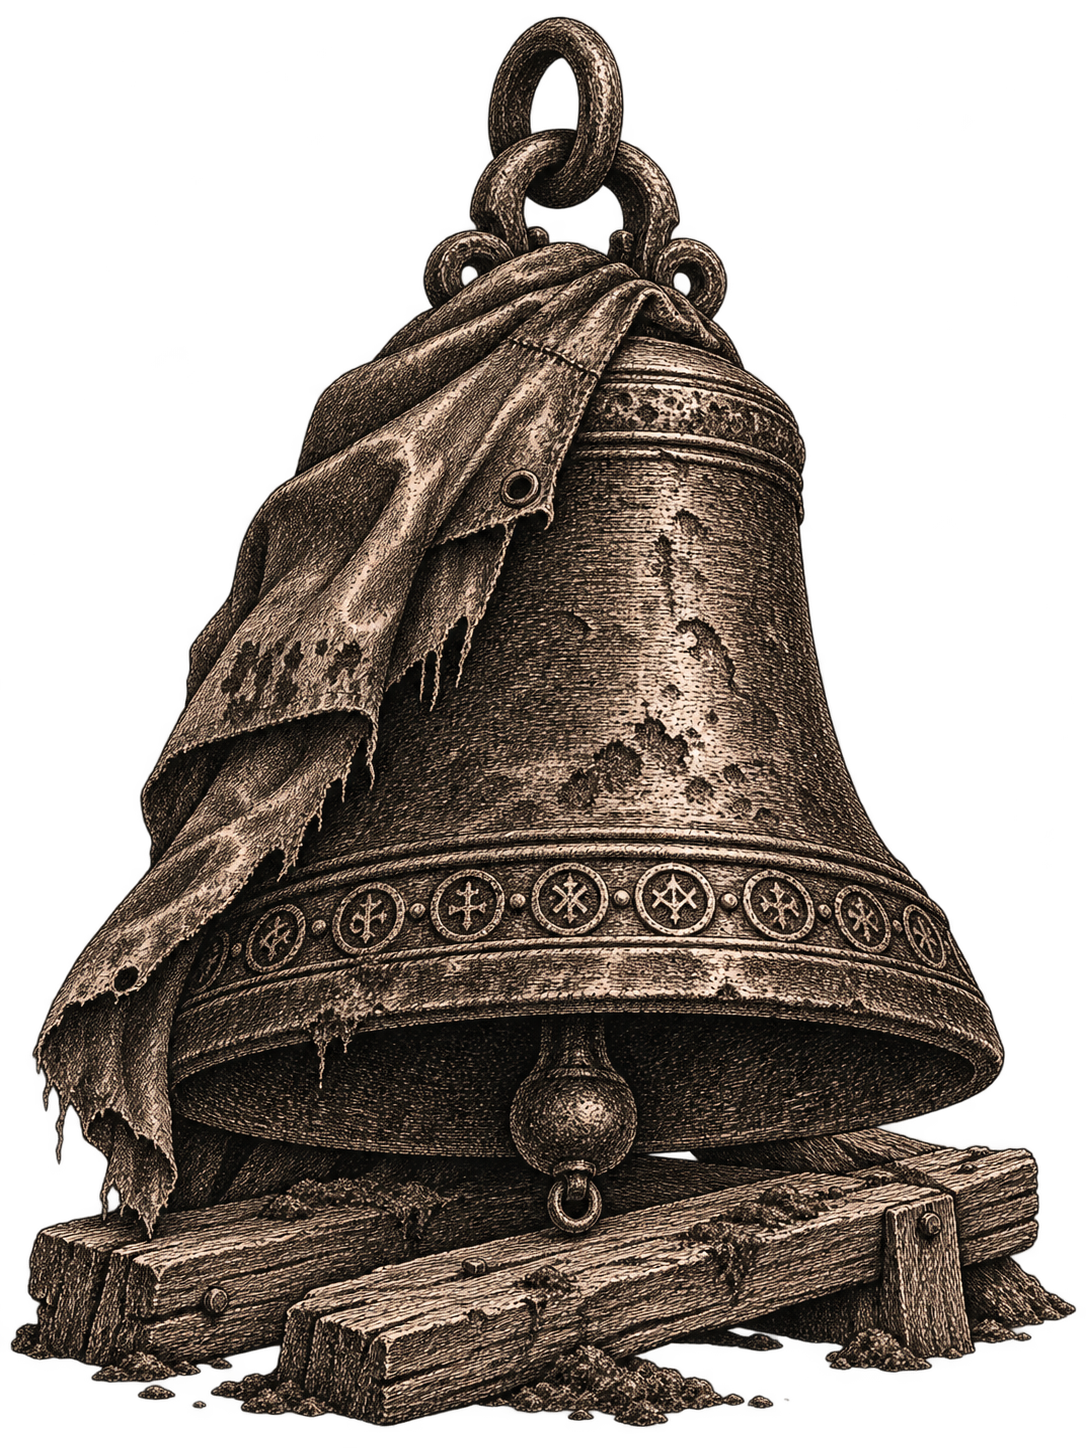
\includegraphics[width=.98\linewidth,height=58mm,keepaspectratio]{assets/hollow-hearth/bell.png}\par{\scriptsize\itshape\color{rpgbrown}La campana robada, envuelta en hule}\vspace{-5pt}\end{wrapfigure}

Hace siete generaciones, un Místico errante llamado \textbf{Veyl Ashen} bendijo una campana de bronce fundida en la fragua de un pequeño asentamiento, levantado donde termina el camino del rey y comienza el bosque antiguo. El asentamiento recibió el nombre de \textbf{Hogar Hueco}. La campana, tañida cada atardecer, mantenía a \textbf{la Gente Hueca} (seres pálidos con piel de corteza que susurran desde entre los árboles) allá abajo, entre las raíces, donde le corresponde estar.

Hace tres noches robaron la campana.

Una banda de forajidos dirigida por un desertor llamado \emph{«Sir»} \textbf{Corwin Vask} bajó de las ruinas de la atalaya donde acampa, mató al aprendiz del viejo campanero y desapareció hacia el norte, bosque adentro, con la campana envuelta en hule. Los aldeanos enterraron al muchacho ayer por la mañana.

La próxima noche sin luna llegará dentro de \textbf{cuarenta y ocho horas}.

Ese es el plazo. Esa noche, cuando se ponga la luna, si ninguna campana suena al anochecer, la Gente Hueca volverá a un Hogar Hueco que ha olvidado cómo defenderse.

\par\vspace{3pt}

\subsection{El gancho}\label{el-gancho}

\begin{wrapfigure}{r}{.38\linewidth}\vspace{-5pt}\centering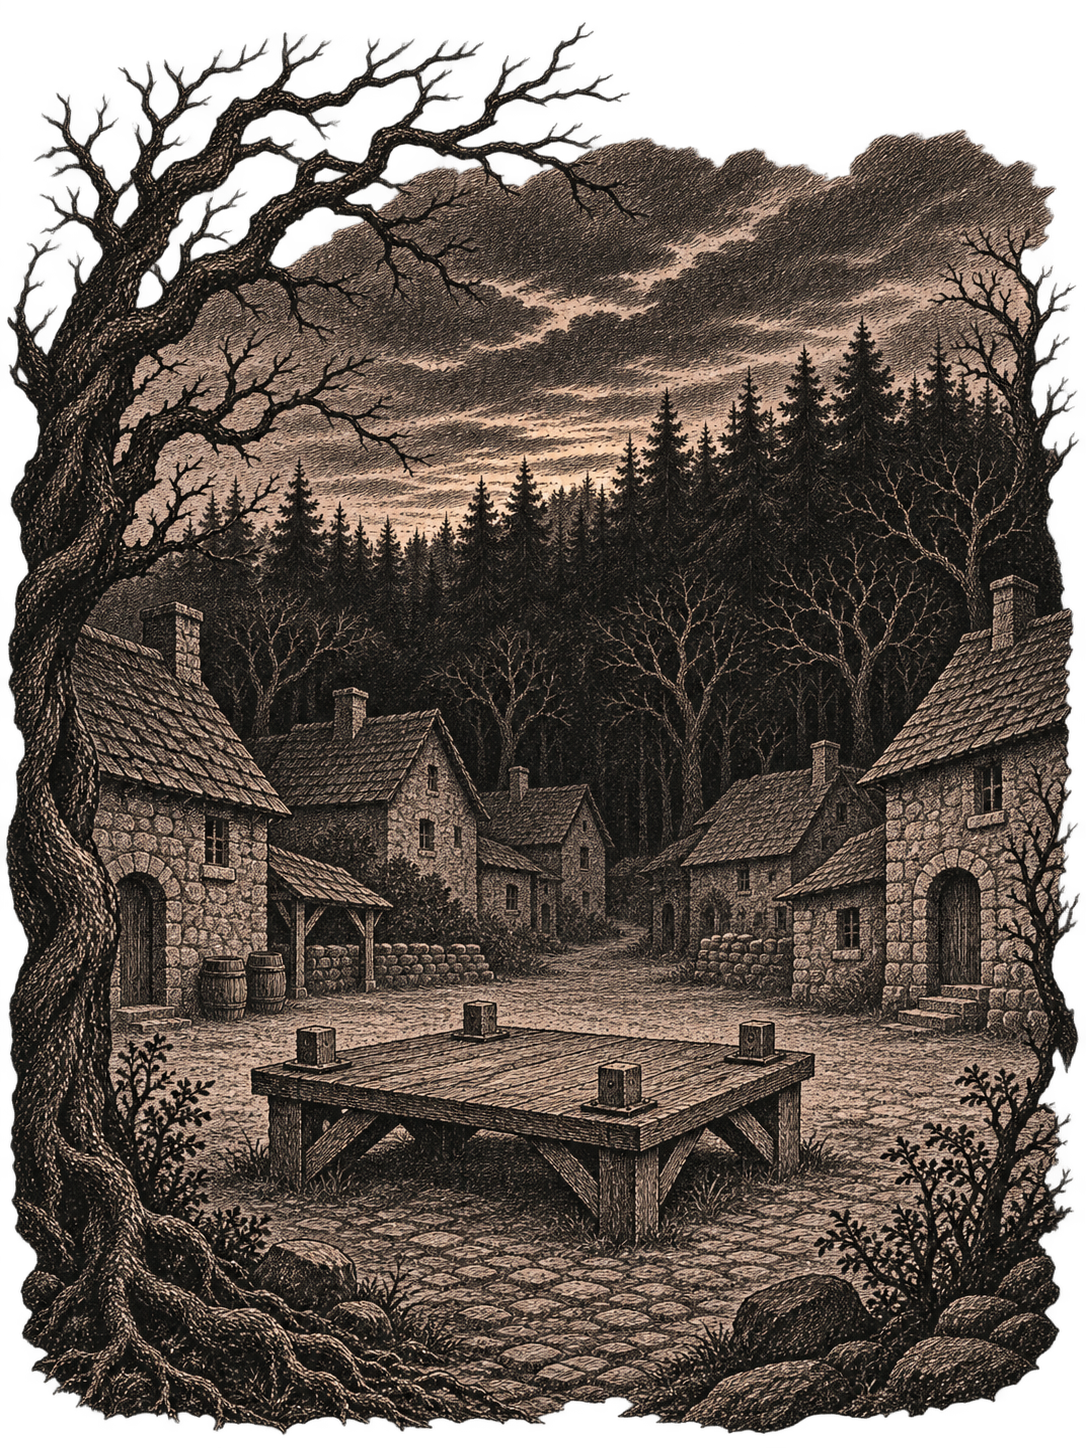
\includegraphics[width=.98\linewidth,height=58mm,keepaspectratio]{assets/hollow-hearth/village.png}\par{\scriptsize\itshape\color{rpgbrown}Hogar Hueco al anochecer: la plataforma vacía}\vspace{-5pt}\end{wrapfigure}

Adapta la llegada a los Rasgos y Cargas que hayan escrito tus jugadores. Algunas ideas rápidas:

\begin{itemize}
\tightlist
\item
  Un \textbf{Erudito} que sigue el linaje de Veyl Ashen en antiguos registros litúrgicos.
\item
  Un \textbf{Aventurero} que trae un contrato del siguiente pueblo del camino.
\item
  Un \textbf{Místico} que \emph{sintió} enmudecer la campana a leguas de distancia.
\item
  Un \textbf{Guerrero} que se aleja de un campo de batalla en el que ya no quiere estar.
\end{itemize}

Lleguen como lleguen, la alcaldesa, \textbf{Hesta Thrush}, les ofrecerá lo poco que tiene Hogar Hueco (monedas, hospitalidad y una reliquia guardada desde la fundación; consulta \emph{Resolución}) a cambio de devolver la campana a casa.

\begin{quote}
\subsubsection{Para leer en voz alta --- La llegada}\label{para-leer-la-llegada}

\emph{El camino se estrecha hasta volverse pista; la pista, sendero; y el sendero desemboca en un claro de casas bajas de piedra con empinados tejados de pizarra. En el centro de la plaza se alza una plataforma de madera. Vacía. Cuatro pernos de hierro, allí donde arrancaron algo pesado. No sale humo de las chimeneas. No hay nadie en la plaza.}

\emph{Entonces se abre una puerta, sale una anciana y, detrás de ella, podéis oír a alguien llorar.}
\end{quote}

\par\vspace{3pt}

\HHSceneMap{map-village}{Hogar Hueco: plano de la aldea}{La plataforma de la campana está en la plaza; Hesta, Bram, Vela y la posada quedan cerca. Todos los lugares de la aldea: Cerca.}
\RPGChapter{Escena 1 --- La aldea}\label{escena-1-la-aldea}

\textbf{Enfoque mecánico:} tiradas de Saber, bonificaciones de Habilidad, tiradas enfrentadas, uso del Rasgo y la Carga.

En Hogar Hueco hay tres personas que importan para vuestra investigación. Los Protagonistas pueden hablar con las tres, en cualquier orden. Cada una tiene una pieza del rompecabezas, y al menos una de ellas \emph{casi} miente.

\par\smallskip\begin{rpgnote}[fontupper=\normalfont]\textbf{Personajes de la aldea}\par\smallskip
\textbf{Hesta Thrush} \emph{(PNJ)} --- Saber Competente. Sin estadísticas de combate; si la violencia la alcanza, es exactamente lo que parece.\par\smallskip
\textbf{Vela Roan} \emph{(PNJ)} --- Saber Experto (Herboristería, Supervivencia), Prodigio Competente. No lucha a menos que la acorralen.\par\smallskip
\textbf{El viejo Bram} \emph{(PNJ)} --- Saber Competente. Ya no puede combatir.\end{rpgnote}\par\smallskip
Consulta \textbf{el plano de la aldea de Hogar Hueco} para ver su distribución. Todos los lugares de la aldea están \textbf{Cerca} unos de otros.

\subsubsection{Hesta Thrush --- La alcaldesa}\label{hesta-thrush-la-alcaldesa}

Una mujer de unos sesenta años, agrietada por la intemperie, consumida por el dolor. Su hijo marchó a la guerra y nunca volvió; lleva once años como alcaldesa y conoce a todos los aldeanos por su segundo nombre.

Lo que cuenta sin reparos:

\begin{itemize}
\tightlist
\item
  Los forajidos vinieron de \textbf{la antigua atalaya}, a cuatro horas de marcha hacia el norte, en el interior del bosque susurrante.
\item
  Como recompensa final de la aldea, ofrece una reliquia de la fundación: la \textbf{Hoja de sal} \emph{(manual, pág. 9)}.
\end{itemize}

Sobre qué mentirá:

Sabe que a su primo \textbf{Marrel} lo vieron bebiendo con uno de los forajidos en la posada la semana antes del robo. No quiere que cuelguen a su primo por ello. Una \textbf{tirada de Saber enfrentada al Saber (Competente) de Hesta} detecta su incomodidad. \textbf{Diplomacia} la convence para que confiese; \textbf{Retórica}, también. \textbf{Intimidación, NO 5}, también funciona, pero pone a la aldea en contra del grupo durante el resto de la aventura.

\begin{quote}
\subsubsection{Gancho para Rasgo/Carga}\label{gancho-para-rasgo-y-carga}

Un Protagonista cuya Carga tenga que ver con la guerra, con hijos perdidos o con juramentos rotos encontrará en Hesta una aliada o un espejo. Aprovéchalo. \emph{«Me recuerdas a él»}, dice, mirando a la persona equivocada.
\end{quote}

\subsubsection{El viejo Bram --- El campanero}\label{el-viejo-bram-el-campanero}

El campanero, de más de ochenta años, sobrevivió porque estaba aliviándose entre las zarzas cuando llegaron los forajidos. El muchacho asesinado era su aprendiz y su sobrino nieto. Está furioso. No a gritos. De la otra manera.

Lo que vio:

\begin{itemize}
\tightlist
\item
  Cuatro hombres. Uno con armadura, uno con arco largo y dos con dagas.
\item
  El de la armadura llevaba \textbf{un sol blanco bordado en el hombro de la capa}, el blasón de una orden caballeresca deshonrada hace diez años. Una \textbf{tirada de Saber, NO 4, con la Habilidad Historia} identifica la orden como la \textbf{Orden del Sol Pálido}, disuelta por «ofensas rituales» durante las guerras. Sin Historia, hace falta \textbf{NO 5} para rescatar un vago recuerdo.
\item
  Cree que la campana está viva. Puede que tenga razón.
\end{itemize}

\subsubsection{Vela Roan --- La herbolaria}\label{vela-roan-la-herbolaria}

Cuarenta años, mente afilada, la única persona de la aldea que ha entrado \emph{en} el bosque susurrante y ha vuelto. Sabe lo que es la Gente Hueca. No lo dirá claramente. Habla con historias.

Lo que ofrece si se le pregunta como es debido:

\begin{itemize}
\tightlist
\item
  La «gente de corteza» sale de las raíces cuando no suena ninguna campana. Cree que un miembro de la Gente Hueca ya camina entre los aldeanos con apariencia mortal.
\item
  Dará un frasco de \textbf{raíz nocturna destilada} (\emph{un objeto notable: vertido sobre una hoja, el siguiente golpe inflige +1 Herida contra criaturas antinaturales; un solo uso}) \textbf{si} un Protagonista acepta traerle una ramita de \textbf{flor de plata lunar} de lo más profundo del bosque.
\end{itemize}

Esto último es una tentación secundaria: una ocasión para un momento de Carga si alguien rompe después su palabra, o para poner a prueba un Rasgo honorable. La flor existe. Que el grupo encuentre tiempo para buscarla depende de ellos.

\subsubsection{Opcional · Marrel, el primo}\label{opcional-marrel-el-primo}

Si los Protagonistas siguen la pista de la mentira de Hesta, pueden encontrar a Marrel en la posada, bebiendo para ahogar el miedo. Confirma que el forajido con quien habló, un hombre llamado \textbf{Thessik}, presumía de un comprador que \emph{«paga en plata del norte»} y que vendría por la campana. Marrel no sabía que iban a robarla. \textbf{Intimidación, NO 4}, lo quiebra. \textbf{Diplomacia, NO 4}, con una copa por medio, también funciona. \textbf{Comercio, NO 4}, si un Erudito quiere desentrañar qué significa en realidad «plata del norte» (es una expresión de los contrabandistas que cruzan la frontera: la plata del norte no existe; es una clave para el oro feérico).

\subsubsection{Momento didáctico para el Narrador}\label{consejo-para-el-narrador}

Cuando un jugador declare \emph{«Quiero saber si miente»}, pregúntale \textbf{cómo}. ¿Presiona? ¿Observa? ¿La pilla en una contradicción? El \emph{cómo} determina el Atributo y la Habilidad. \textbf{Saber} es lo habitual para interpretar a una persona; \textbf{Etiqueta} la sorprende en deslices de cortesía, \textbf{Intimidación} la empuja a cometer errores, \textbf{Engaño} te permite acorralarla mintiendo mejor que ella. No hay un subsistema aparte de combate social. Solo hay Saber más una Habilidad pertinente contra un NO. Igual que en todo lo demás.

\par\vspace{3pt}

\HHSceneMap{map-forest}{A través del bosque susurrante}{La aldea abajo, la torre arriba; la Gente Hueca aparece en la orilla que el grupo acaba de dejar.}

\RPGChapter{Escena 2 --- El bosque susurrante}\label{escena-2-el-bosque-susurrante}

\begin{wrapfigure}{r}{.38\linewidth}\vspace{-5pt}\centering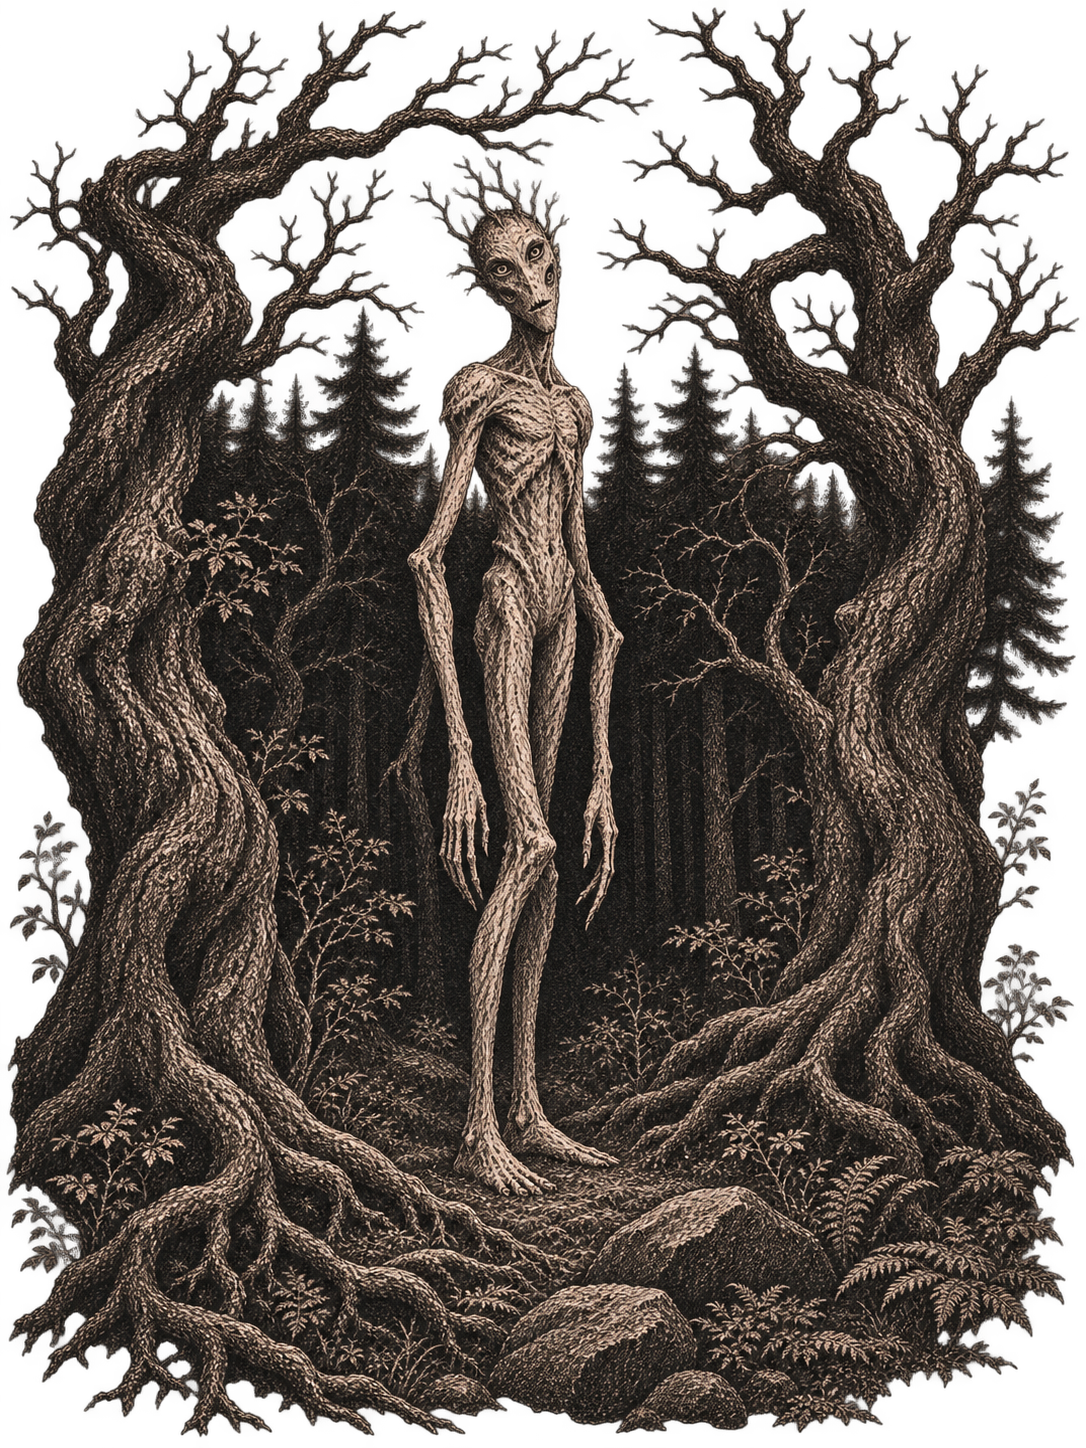
\includegraphics[width=.98\linewidth,height=58mm,keepaspectratio]{assets/hollow-hearth/hollow.png}\par{\scriptsize\itshape\color{rpgbrown}Un observador entre los árboles}\vspace{-5pt}\end{wrapfigure}

\textbf{Enfoque mecánico:} mecánica de Ayuda, categorías de distancia, Condiciones como $-1$ grado.

Un rastro de helechos aplastados y jirones de hule caídos sale de la aldea hacia el norte. El bosque susurrante se lo traga a los cincuenta pasos. Aquí los árboles se inclinan hacia dentro.

\begin{quote}
\subsubsection{Para leer en voz alta --- Entrando en el bosque}\label{para-leer-entrando-en-el-bosque}

\emph{La luz cae un tercio en cuanto cruzáis la linde de los árboles. No por las copas (no hay copas dignas de ese nombre), sino como si el propio aire se la bebiera. El sonido se aplana. Los pasos dejan de oírse a lo lejos. Tras diez minutos de marcha, lo único que podéis oír es vuestra propia respiración y, muy a lo lejos, algo que podría ser el viento entre las ramas o podrían ser voces diciendo algo que no llegáis a entender.}
\end{quote}

Consulta \textbf{el mapa del trayecto por el bosque susurrante}: va de la aldea a la atalaya, con el puente y el punto del Avistamiento señalados.

\subsubsection{El rastro · Una prueba de Supervivencia}\label{el-rastro-prueba-de-supervivencia}

El rastro es real, pero fácil de perder. Un personaje con \textbf{Supervivencia} tira \textbf{Destreza, NO 4}. Un personaje con Destreza Competente y la Habilidad tira 2d6 y conserva el mayor; uno con Destreza Experto sin la Habilidad tira lo mismo; uno con Destreza Inexperto y sin la Habilidad tira 2d6 y conserva el menor, algo nada amable.

Es el momento perfecto para introducir la \textbf{Ayuda} \emph{(manual, pág. 7)}:

\begin{itemize}
\tightlist
\item
  Un \textbf{ayudante competente} (aquel cuya propia tirada en la misma tarea sería de nivel Experto o superior) añade \textbf{+1d6} a la reserva del personaje principal, sin penalización.
\item
  Un \textbf{ayudante incompetente} (cualquiera que tiraría por debajo del nivel Experto en la misma tarea) añade \textbf{+1d6}, \emph{pero aumenta el NO en 1}. Un Guerrero que «ayuda» ruidosamente al Aventurero a seguir el rastro puede empeorar las cosas.
\end{itemize}

Deja que los jugadores lo vean ocurrir. Un Guerrero que ayuda al rastreador convierte el NO 4 en NO 5, y luego comprende la lección cuando se pierde el rastro.

Si se pierde el rastro, pasa una hora más y el anochecer sorprende al grupo en el bosque. Desde ese momento hasta el amanecer, todas las tiradas sufren una \textbf{Condición: $-1$ grado}.

\subsubsection{El puente podrido}\label{el-puente-podrido}

El rastro cruza un barranco por un puente de un solo tronco que nadie ha cuidado en veinte años. El tronco solo aguanta a una persona cada vez. Debajo hay una caída de unos quince metros hasta un arroyo que corre entre rocas.

\begin{itemize}
\tightlist
\item
  \textbf{Tirada de Destreza, NO 4}, para cruzar sin percances. Con \textbf{Acrobacias}, sin apuros.
\item
  Quien cae sufre \textbf{2 Heridas} (de combate, por las rocas). Una \textbf{tirada de Medicina, NO 4}, durante la escena, recupera 1 Herida (2 con un Crítico).
\item
  Una cuerda tendida como pasamanos (\textbf{Fuerza + Artesanía o + Resistencia, NO 3}) reduce el NO de todos a 3 y elimina la consecuencia del fallo.
\end{itemize}

También es una prueba discreta del Rasgo. Un Protagonista cuyo Rasgo diga \emph{«No dejo a nadie atrás»}, que falle su propia tirada para cruzar y al que luego un compañero tenga que ayudar a pasar, debería sentirlo.

\subsubsection{El Avistamiento}\label{el-avistamiento}

Crucen bien o mal, cuando \textbf{la última persona llega al otro lado}, \textbf{un miembro de la Gente Hueca} aparece entre dos árboles en la orilla que acaban de dejar. Pálido. Con piel de corteza. Un poco demasiado alto. La boca no está exactamente donde debería estar una boca. No se mueve. No amenaza. Los mira alejarse. Al cabo de treinta segundos, ha desaparecido.

Es solo ambiente. No hay tirada. Deja que los jugadores se queden con esa sensación.

\begin{quote}
\subsubsection{Momento didáctico --- Distancias}\label{consejo-distancias}

La criatura hueca está \textbf{Lejos} (al otro lado del barranco, fuera del alcance razonable de un arco). Un Místico con un Grimorio de percepción (\emph{Ojo del vacío}, manual, pág. 11, por ejemplo) puede querer verla más de cerca. Permíteselo. Hazle pagar el coste de Fatiga. Muestra a la mesa cómo es una tirada de Prodigio cuando lo único en juego es el conocimiento.
\end{quote}

\subsubsection{Los lobos · Encuentro opcional de ajuste}\label{los-lobos-encuentro-opcional}

Si la sesión avanza deprisa y el grupo parece poco puesto a prueba, una pareja de \textbf{lobos hambrientos} puede emboscarlo en el último tramo antes de la atalaya. Dos lobos enseñan la regla de \textbf{enemigos en grupo} (manual, pág. 12) y permiten que el Guerrero golpee por primera vez. \par\smallskip\begin{rpgnote}[fontupper=\normalfont]\textbf{Lobo hambriento} \emph{(encuentro opcional del bosque)} \emph{NO Fue3/Des4 · Competente · 2 Heridas · mordisco (2H Fue.).} \emph{Comportamiento: «Caza al más débil. Tres noches sin comer».}\end{rpgnote}

\par\vspace{3pt}

\RPGChapter{Escena 3 --- La antigua atalaya}\label{escena-3-la-antigua-atalaya}

\begin{wrapfigure}{r}{.38\linewidth}\vspace{-5pt}\centering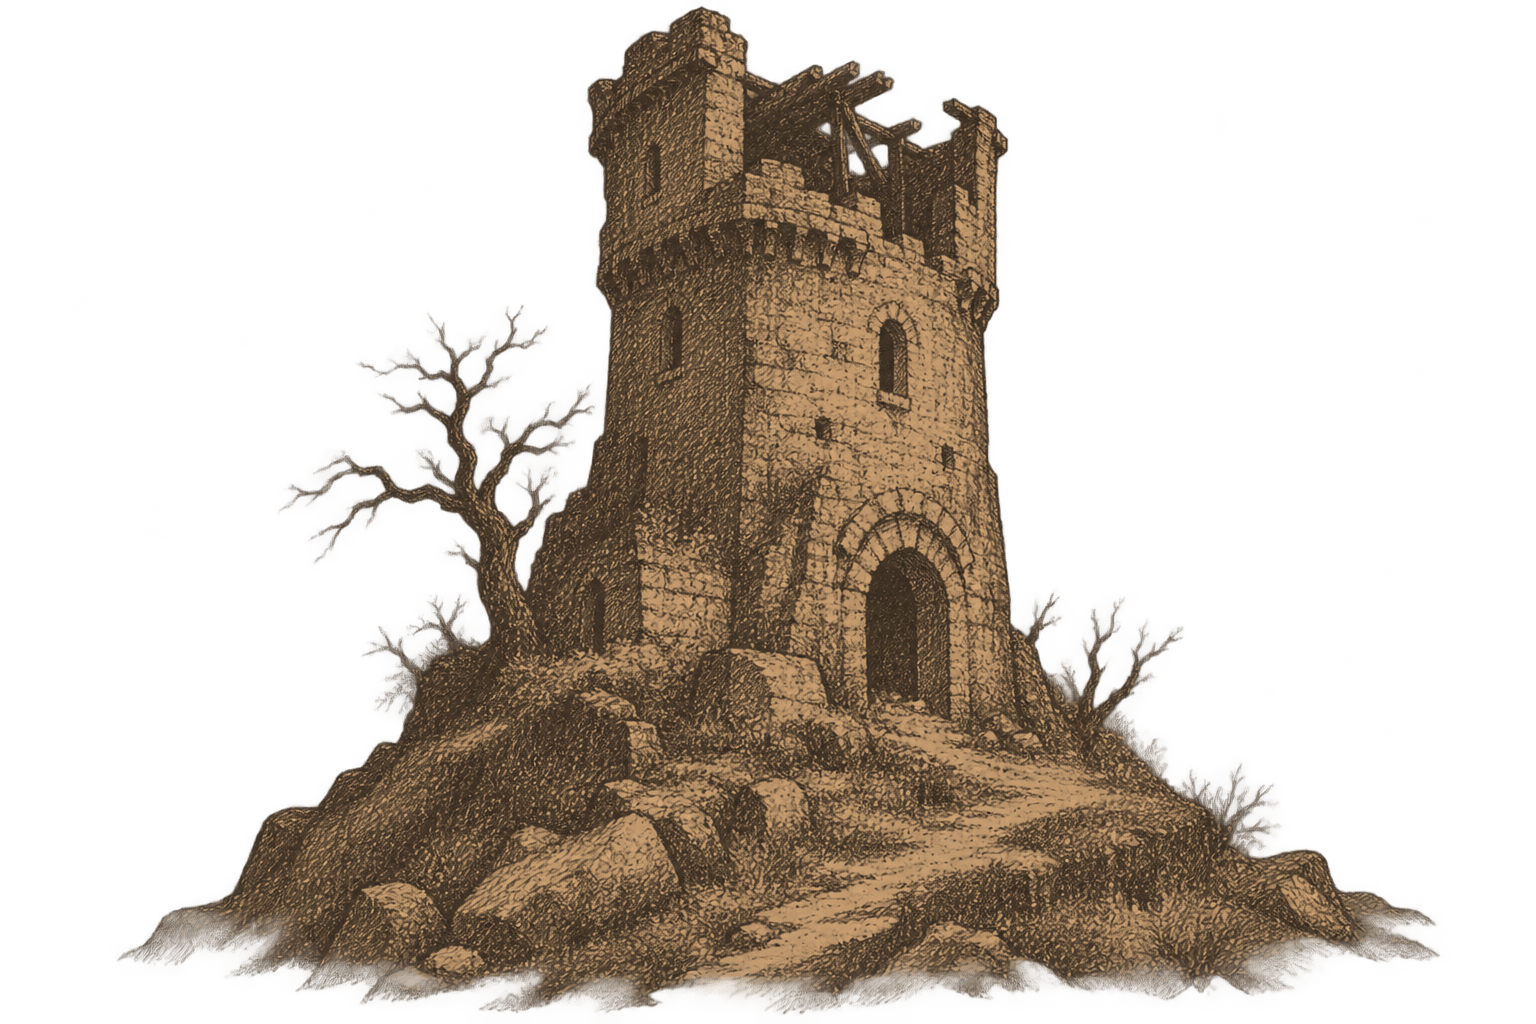
\includegraphics[width=.98\linewidth,height=58mm,keepaspectratio]{assets/hollow-hearth/tower.png}\par{\scriptsize\itshape\color{rpgbrown}La antigua atalaya al anochecer}\vspace{-5pt}\end{wrapfigure}

\textbf{Enfoque mecánico:} combate como conversación, Heridas y Fatiga, Crítico, Reacción adversa, \textbf{Esfuerzo}.

La antigua atalaya tiene dos pisos de piedra carcomida sobre una pequeña loma; ha perdido la mitad del tejado y la hiedra crece en las grietas. Frente a la entrada brilla una hoguera. Junto a ella están sentados dos forajidos. Dentro, en el piso inferior, duermen otros dos. En el piso superior, \textbf{Sir Corwin Vask} espera a su comprador sentado junto a la campana envuelta en hule.

El comprador llegará \textbf{a medianoche}. Ahora está anocheciendo.

Consulta \textbf{el plano del piso inferior de la atalaya} para el piso inferior y sus accesos, y \textbf{el plano del piso superior de la atalaya} para la distribución del piso superior, donde tiene lugar el clímax.
\HHInlineFigure{map-ground}{.68}{Antigua atalaya: piso inferior --- entrada y hoguera al sur, muro derrumbado al oeste, escalera al norte.}

\par\smallskip\begin{rpgnote}[fontupper=\normalfont]\textbf{Forajidos}\par\smallskip \textbf{Forajido} \emph{NO Fue3/Des3 · Competente · 2 Heridas · daga (2H Des.) o garrote corto (1F Fue.).} \emph{Comportamiento: «Cobardes en un combate justo. Huyen si Corwin cae».} \emph{En grupo: una sola tirada, +1H por cada miembro además del primero (máximo +3). Cada Herida infligida al grupo elimina a un miembro.}\end{rpgnote}\par\smallskip
\subsubsection{Tres aproximaciones}\label{tres-opciones}

El grupo tiene opciones. Antes de cualquier tirada, pregunta sin rodeos: \emph{«¿Cómo queréis hacerlo?»}. Las mecánicas cambian en consecuencia.

\textbf{Sigilo.} El muro derrumbado del lado oeste se descubre con una \textbf{tirada de Saber + Táctica, NO 3}, o simplemente describiéndolo. Cada personaje tira \textbf{Destreza + Sigilo, NO 4}, para acercarse sin ser visto. Un fallo alerta a los dos forajidos de la hoguera. Dos fallos alertan a todos, Corwin incluido. Una aproximación limpia permite al grupo llegar al piso superior y sorprenderlo.

\par\Needspace{10\baselineskip}\noindent\textbf{Parlamento.} Acercarse a la hoguera y hablar. Corwin es un hombre de orgullo roto. Si un Protagonista (sobre todo el Guerrero) se dirige a él como \emph{«Sir Corwin»}, su Carga se resquebraja. \textbf{Saber + Diplomacia o Retórica, NO 5}, lo convence de \emph{plantearse} devolver la campana a cambio de un precio en lugar de vendérsela al comprador. Exigirá más que la recompensa de la aldea, pero el grupo puede prometérselo. Mentirle sobre la recompensa es una \textbf{tirada de Saber + Engaño enfrentada a su Saber (Competente)}.

\textbf{Asalto.} Entrar luchando. Dos forajidos junto al fuego, dos dentro, Corwin arriba. Ruidoso, sangriento y la forma más directa de enseñar el combate a jugadores nuevos.

\par\smallskip\begin{rpgnote}[fontupper=\normalfont]\textbf{Sir Corwin Vask, caballero caído en desgracia} \emph{NO Fue4/Des5 · Experto · 6 Heridas · espada larga (2H Fue.) · armadura pesada.} \emph{Comportamiento: «No golpea a un hombre de rodillas. Se batirá en duelo con cualquiera que lo llame “sir”. Odia a los Místicos: así se lo enseñó su orden».} \emph{Opcional: lleva un medallón gastado con el retrato de su hermana. Si un Protagonista lo ve durante el combate, dale ocasión de usarlo.}\end{rpgnote}\par\smallskip
\subsubsection{El piso superior}\label{el-piso-superior}

La campana, Sir Corwin y el enfrentamiento decisivo están en el piso superior. Su distribución importa, porque de ella dependen las decisiones tácticas de los jugadores.

\par\medskip\noindent
\begin{tabular}{@{}p{.60\linewidth}@{\hspace{.028\linewidth}}p{.345\linewidth}@{}}
\centering\vspace{0pt}
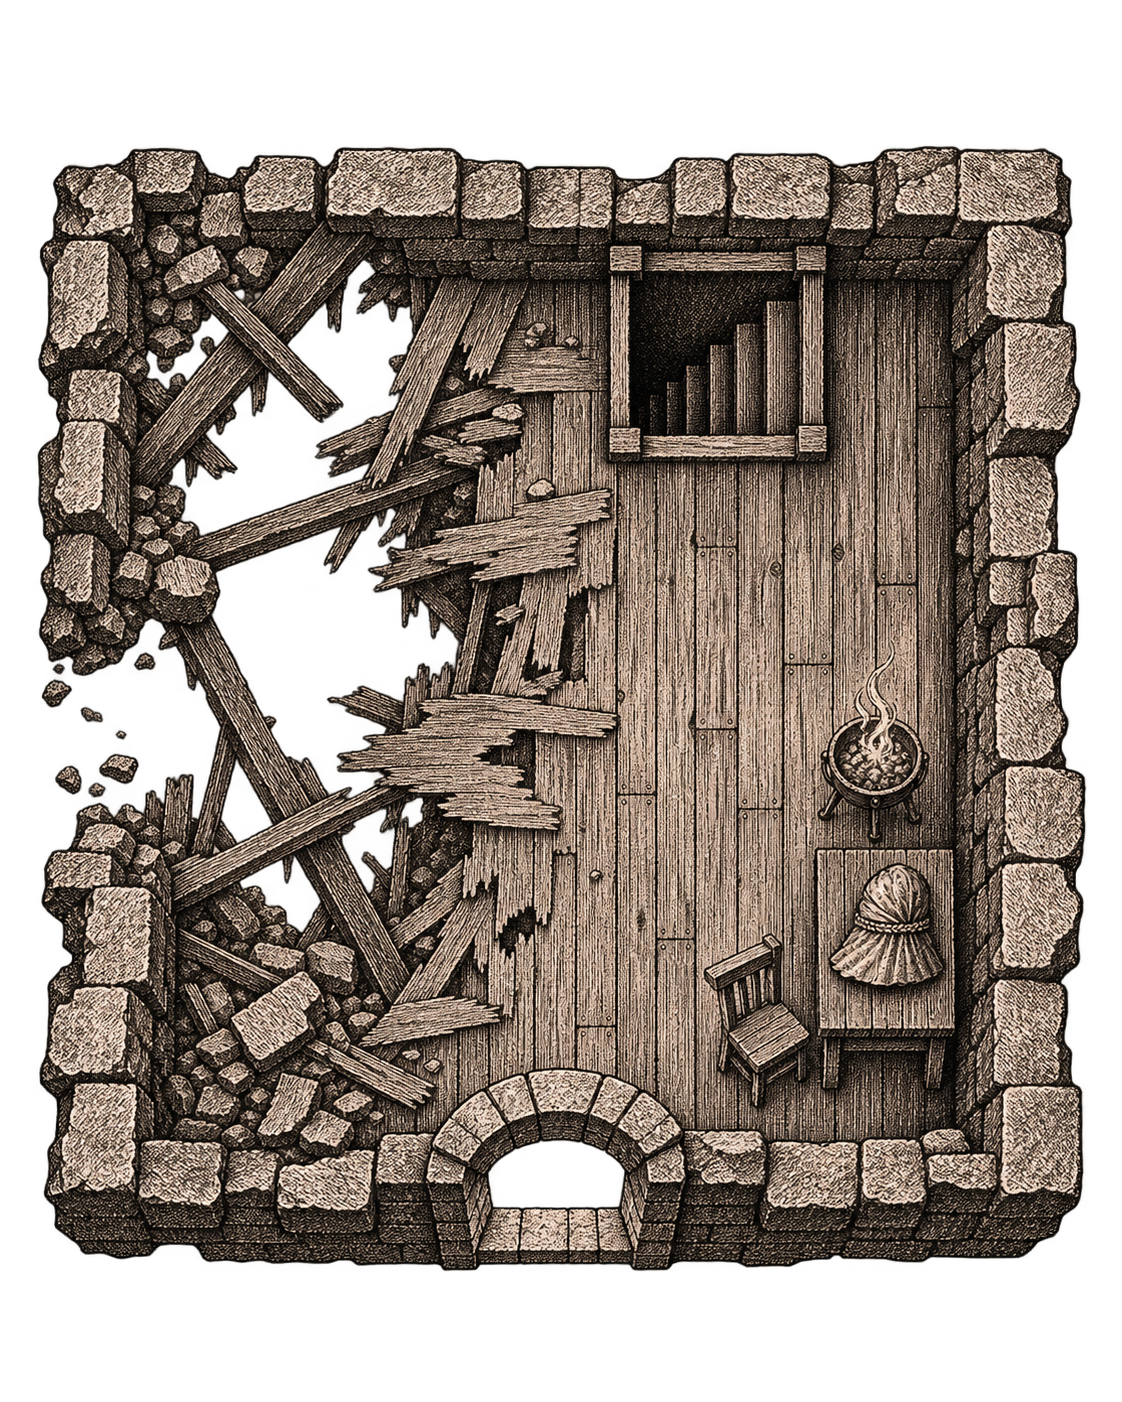
\includegraphics[width=.98\linewidth,height=70mm,keepaspectratio]{assets/hollow-hearth/map-upper.png}\par\vspace{2pt}
{\footnotesize\itshape\color{rpgbrown}Antigua atalaya: piso superior\par}
{\scriptsize Escalera al norte; lado occidental a cielo abierto; ventana sur, campana y brasero en el lado este, intacto.\par}
&
\centering\vspace{0pt}
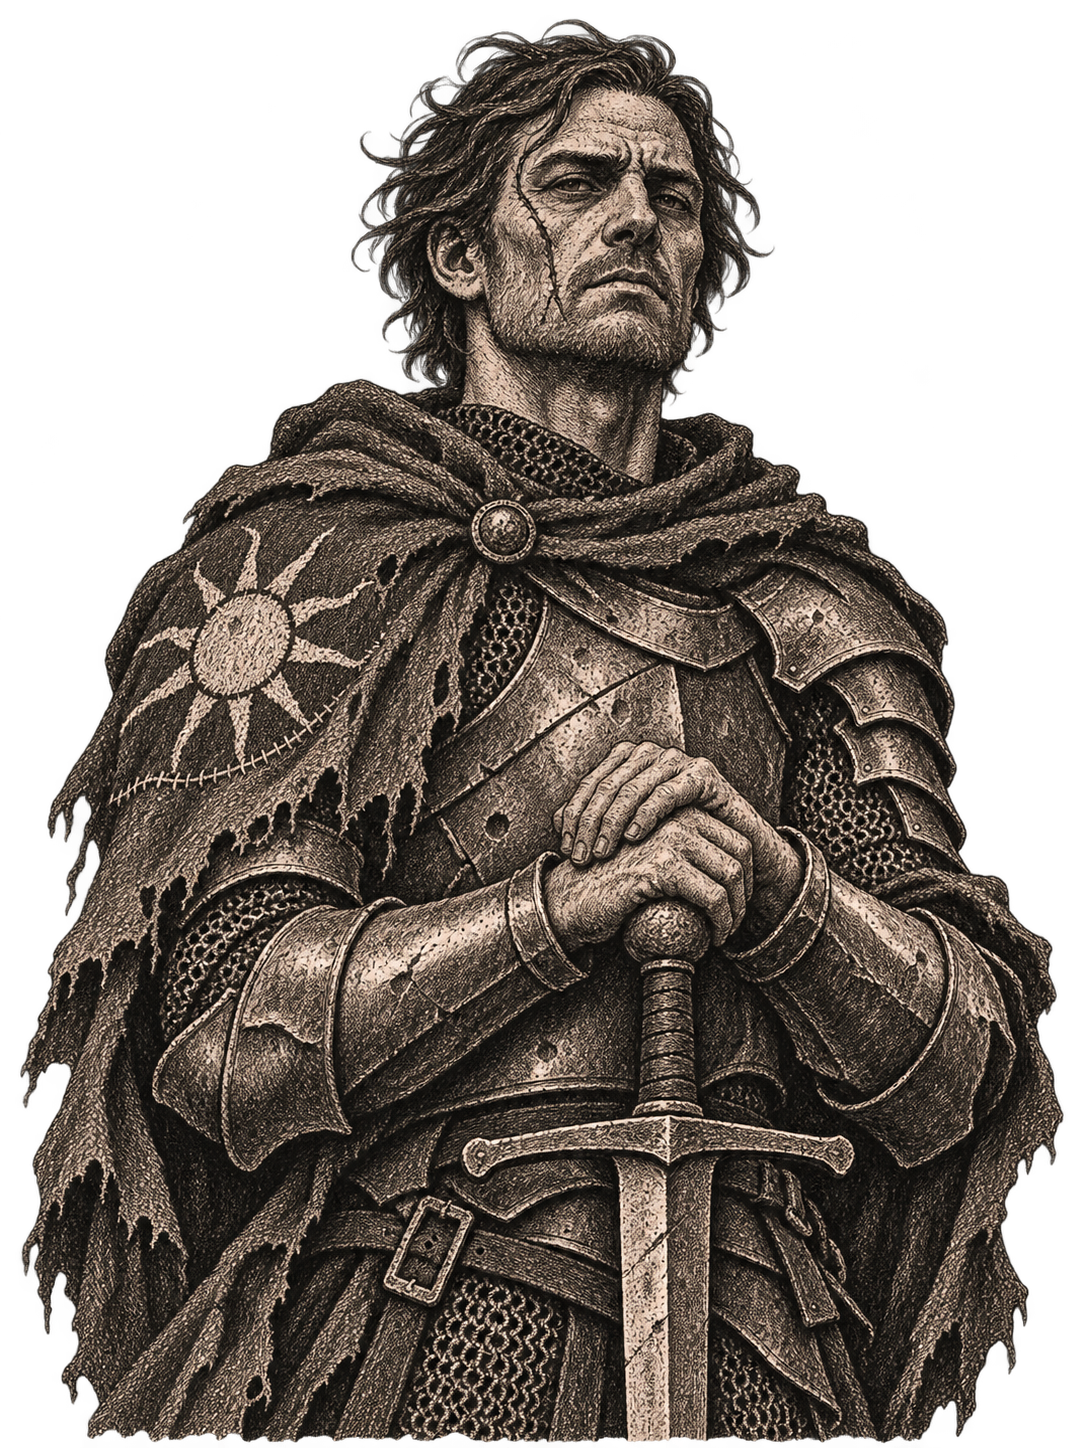
\includegraphics[width=.95\linewidth,height=68mm,keepaspectratio]{assets/hollow-hearth/corwin.png}\par\vspace{2pt}
{\footnotesize\itshape\color{rpgbrown}Sir Corwin Vask\par}
\end{tabular}
\par\medskip

Sir Corwin está sentado en una silla de madera junto a \textbf{la ventana sur}, vigilando el sendero por el que subirá el comprador. La campana está a su lado, sobre una mesita, todavía envuelta en hule embarrado. Un brasero de rescoldos da la única luz cálida de la estancia. La escalera desemboca junto al muro norte, \textbf{a sus espaldas}.

\textbf{La mitad occidental del piso superior está a cielo abierto}: el mismo derrumbe que se llevó el muro occidental del piso inferior arrastró la parte occidental del tejado y parte del suelo occidental. Hay vigas sueltas colgando en ángulo. El suelo occidental expuesto no es seguro si se camina sin cuidado.

Esto crea una \textbf{cuarta aproximación} que hasta ahora solo se insinuaba:

\textbf{La escalada.} Un personaje con \textbf{Acrobacias} puede trepar por el montón de cascotes del muro derrumbado del piso inferior y seguir subiendo por el exterior de la pared occidental rota, hasta entrar por el hueco del tejado. Tira \textbf{Destreza + Acrobacias, NO 4}, para trepar limpiamente; sin Acrobacias, \textbf{NO 5}. Un fallo significa caer: 1 Herida por la altura, más el ruido de la caída (Corwin lo oirá). Con un éxito, el personaje cae en el piso superior \emph{a espaldas} de Corwin, por sorpresa. Es una aproximación para un solo personaje: el Guerrero con armadura pesada no puede hacer esta escalada, y el Místico de 2 PV no puede permitirse la caída si falla. \textbf{Un Aventurero ágil es el más indicado para esta aproximación.}

\par\Needspace{12\baselineskip}\noindent\textbf{Elementos tácticos del piso superior:}

\begin{itemize}
\tightlist
\item
  \textbf{La ventana sur.} Quien llegue a la campana puede arrojarla por ella: cae con fuerza cerca de la hoguera, quizá agrietada. El comprador, que vigila desde el sendero, lo verá. Un Protagonista también puede usar la ventana para huir de la estancia saltando al suelo (Destreza + Acrobacias, \textbf{NO 4}, para caer bien; un fallo cuesta 1 Herida).
\item
  \textbf{La mitad occidental inestable.} Todo combate que tenga lugar en la mitad derrumbada sufre una Condición: \textbf{$-1$ grado}. Un personaje empujado por el borde cae un piso (2 Heridas). Corwin, que conoce la estancia, solo luchará en la mitad oriental, e intentará con gusto empujar a sus enemigos hacia el suelo inseguro.
\item
  \textbf{El brasero.} Si se vuelca, las brasas se esparcen por el suelo de madera seca: el fuego se extiende durante el equivalente a dos escenas de acción y la estancia se vuelve inhabitable. Una maniobra desesperada, al alcance de cualquiera, que puede salvar al grupo o destruir la campana junto con todo lo demás.
\item
  \textbf{La armadura pesada de Sir Corwin.} Su armadura pesada fija el NO para golpearlo en \textbf{4 con Fuerza} o \textbf{5 con Destreza}. No reduce el daño. Un brasero volcado, un empujón hacia el borde derrumbado o un Crítico de un Protagonista que haya declarado Esfuerzo pueden cambiar el enfrentamiento.
\end{itemize}

\subsubsection{Ajustar el encuentro}\label{ajustar-el-encuentro}

\begingroup\setlength{\arrayrulewidth}{.34pt}\arrayrulecolor{rpgline}\renewcommand{\arraystretch}{1.32}\rowcolors{2}{rpgshade}{white}\par\smallskip\noindent\begin{tabularx}{\linewidth}{|Y|Y|Y}\hline
\rpghead{Tamaño del grupo} & \rpghead{Forajidos} & \rpghead{Sir Corwin} \\ \hline
3 jugadores & 3 forajidos (en grupo) & Sí \\ \hline
4 jugadores & 4 forajidos (2 fuera, 2 dentro) & Sí \\ \hline
\end{tabularx}\arrayrulecolor{black}\endgroup\par\smallskip

Si el grupo parece pasarlo muy mal, haz que un forajido huya a la primera señal de sangre de verdad. Si lo están superando sin esfuerzo, el comprador llega antes de tiempo.

\subsubsection{El giro · El comprador}\label{el-giro-el-comprador}

Si el grupo sigue en la atalaya a \textbf{medianoche} (en mitad del combate, hablando o tras haber vencido), una figura con túnica sale del bosque, sola, sin rostro bajo la capucha. \textbf{El comprador es un miembro de la Gente Hueca con apariencia mortal.} Quiere silenciar la campana para siempre, no destruirla. Lleva una bolsita de plata. Habla con las mismas voces no del todo correctas que el grupo oyó a medias al entrar en el bosque.

\par\smallskip\begin{rpgnote}[fontupper=\normalfont]\textbf{El comprador (miembro de la Gente Hueca con apariencia mortal)} \emph{NO Fue3/Des4 · Experto · 4 Heridas · toque (1F Prodigio; con un Crítico, 2H + una Condición que dura el resto de la escena) · sin armadura.} \emph{Comportamiento: «Pronuncia las sílabas equivocadas. Los árboles no responden. Sangra savia, no sangre».}\end{rpgnote}\par\smallskip
Es un \textbf{momento de elección}. El grupo puede:

\begin{itemize}
\tightlist
\item
  \textbf{Negarse y luchar.} \emph{(Estadísticas más arriba.)}
\item
  \textbf{Aceptar la plata.} El grupo se marcha rico. Nadie vuelve a ver Hogar Hueco con vida. \emph{Si lo eligen, deja que sea un final de verdad.}
\item
  \textbf{Mentir y tender una emboscada al comprador.} \textbf{Tiradas enfrentadas de Saber contra el Saber (Experto) del comprador}. Si el grupo gana, conserva la plata \emph{y} la campana, pero el bosque lo ha marcado, y la siguiente aventura empieza con esa marca.
\end{itemize}

\subsubsection{El clímax --- y la última tirada}\label{el-cluxedmax-la-uxfaltima-tirada}

Sea cual sea el camino elegido, el momento culminante debería dejar al menos a un Protagonista en estado \textbf{Malherido} o \textbf{Grave}. Vigila los PV en la mesa. En el instante en que un jugador baje a \textbf{1 PV} y aún tenga que tirar para cerrar la escena, haz una pausa. Míralo desde el otro lado de la mesa. Pregunta:

\begin{quote}
\emph{«Todo se decide a la última tirada. ¿Quieres sangrar por ello?»}
\end{quote}

Guíalo para declarar \textbf{Esfuerzo} \emph{(manual, pág. 13)}. Deja que tire; la Herida de Fatiga llega después de la tirada. \textbf{Este es el momento que da nombre al juego.} Haz que se note. Si la tirada tiene éxito, la mesa debería estallar en vítores. Si falla, la mesa debería quedarse en silencio.

\par\vspace{3pt}

\subsection{Resolución}\label{resoluciuxf3n}

Tres desenlaces claros, con consecuencias que siembran la siguiente aventura:

\textbf{La campana regresa.} Hesta entrega la \textbf{Hoja de sal} y toda la hospitalidad de la aldea. Si se le trajo su flor, Vela cuenta al grupo entre sus amigos. La noticia llega al pueblo vecino. \emph{La siguiente aventura comienza cuando alguien busca al grupo por su nombre.}

\textbf{La campana es silenciada o vendida.} El grupo se marcha rico y marcado. La Gente Hueca toma nota. \emph{Una futura aventura comienza con susurros nocturnos que conocen sus nombres.}

\textbf{La campana es destruida.} Ya sea por una Reacción adversa desafortunada o por una lucha desesperada, la Gente Hueca vuelve a Hogar Hueco en la noche sin luna. \emph{La siguiente aventura comienza con el grupo intentando remediarlo. Puede que Veyl Ashen, el Místico original, no esté tan muerto como dicen las crónicas.}

\subsubsection{Las tres preguntas}\label{las-tres-preguntas}

Termina la sesión haciendo que el grupo responda en conjunto a las tres preguntas de Avance (manual, pág. 11). Lo correcto es un recuento sincero, no generoso. Un jugador nuevo que se bloqueó a cada paso no ha ganado puntos de avance. Un jugador nuevo que lo intentó, fracasó y afrontó las consecuencias ha ganado tres. Déjalo claro, con delicadeza, la primera vez.

\par\vspace{3pt}

\par\smallskip\section*{Referencia rápida del Narrador}\label{referencia-ruxe1pida-del-narrador}\addcontentsline{toc}{section}{V. Referencia rápida del Narrador}
\begingroup\footnotesize\setlength{\arrayrulewidth}{.34pt}\arrayrulecolor{rpgline}\renewcommand{\arraystretch}{1.14}
\noindent\begin{minipage}[t]{.49\linewidth}
\begin{tabularx}{\linewidth}{|>{\hsize=.78\hsize}Y|>{\hsize=1.22\hsize}Y|}\hline
\rpghead{Situación} & \rpghead{Regla / objetivo} \\ \hline
NO 3–6 & Sencilla / Normal / Difícil / Extrema \\ \hline
Distancias & Contacto; Cerca; A distancia; Lejos \\ \hline
Ayuda & Experto o más: +1d6; inferior: +1d6 y NO +1 \\ \hline
Esfuerzo & +1d6 antes de tirar; 1F después \\ \hline
Estado & $\le$ 2 PV: $-1$ grado; $\le$ 1 PV: $-2$ grados \\ \hline
\end{tabularx}
\end{minipage}\hfill
\begin{minipage}[t]{.49\linewidth}
\begin{tabularx}{\linewidth}{|>{\hsize=.78\hsize}Y|>{\hsize=1.22\hsize}Y|}\hline
\rpghead{Situación} & \rpghead{Regla / objetivo} \\ \hline
Puente & Destreza NO 4; cuerda NO 3; caída 2H \\ \hline
Rastreo & Destreza + Supervivencia, NO 4 \\ \hline
Sigilo & Destreza + Sigilo, NO 4 \\ \hline
Escalada & Destreza + Acrobacias, NO 4 (si no, 5) \\ \hline
Corwin & NO Fue4/Des5; Experto; 6H; espada 2H \\ \hline
\end{tabularx}
\end{minipage}
\arrayrulecolor{black}\endgroup


\HHAdventureBackCover
\end{document}
